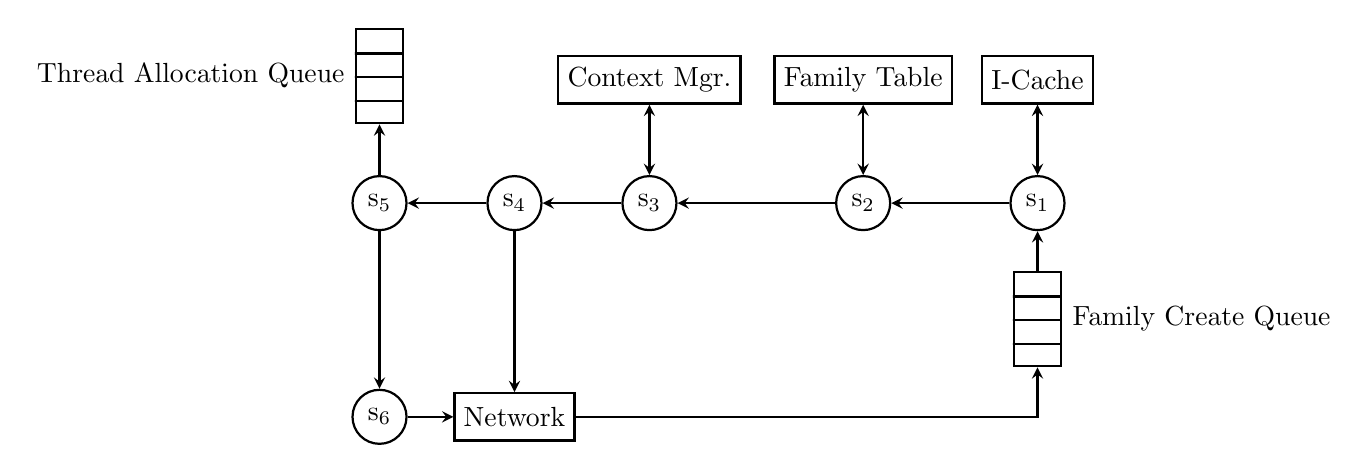
\begin{tikzpicture}[auto,>=stealth,thick,text badly centered]

  % Family allocation queue
  \node[draw,rectangle,minimum width=0.6cm,minimum height=1.2cm] (falloc) {};
  \draw (falloc.south west)+(0,0.3) rectangle +(0.6,0.3);
  \draw (falloc.south west)+(0,0.6) rectangle +(0.6,0.6);
  \draw (falloc.south west)+(0,0.9) rectangle +(0.6,0.9);
   
  \begin{scope}[every node/.style={draw,circle}]
    \node (s1) at (falloc.north) [above=0.5cm] {s$_1$};
    \node (s2) at (s1.west) [left=1.5cm] {s$_2$};
    \node (s3) at (s2.west) [left=2cm] {s$_3$};
    \node (s4) at (s3.west) [left=1cm] {s$_4$};
    \node (s5) at (s4.west) [left=1cm] {s$_5$};
    \node (s6) at (s5.south) [below=2cm] {s$_6$};
  \end{scope}
  \node at (falloc.east) [right] {Family Create Queue};
  
  \draw[->] (falloc) -- (s1);
  \draw[->] (s1) -- (s2);
  \draw[->] (s2) -- (s3);
  \draw[->] (s3) -- (s4);
  \draw[->] (s4) -- (s5);
  \draw[->] (s5) -- (s6);
  
  \begin{scope}[every node/.style={draw,rectangle,minimum height=0.6cm}]
    \node (icache)   at (s1) [above=1.25cm] {I-Cache};
    \node (ft)       at (s2) [above=1.25cm] {Family Table};
    \node (contexts) at (s3) [above=1.25cm] {Context Mgr.};
  \end{scope}
  
  % Thread allocation queue
  \node[draw,rectangle,minimum width=0.6cm,minimum height=1.2cm] (talloc) at (s5) [above=1cm] {};
  \draw (talloc.south west)+(0,0.3) rectangle +(0.6,0.3);
  \draw (talloc.south west)+(0,0.6) rectangle +(0.6,0.6);
  \draw (talloc.south west)+(0,0.9) rectangle +(0.6,0.9);
  \node at (talloc.west) [left] {Thread Allocation Queue};

  % Network
  \node[draw,rectangle,minimum height=0.6cm] (net) at (s6 -| s4) {Network};
  \draw[->] (net) -| (falloc);
  
  \begin{scope}[every node/.style={font=\footnotesize}]
    \draw[<->] (s1) -- (icache);
    \draw[<->] (s2) -- (ft);
    \draw[->]  (s4) -- (net);
    \draw[<->] (s3) -- (contexts);
    \draw[->]  (s5) -- (talloc);
    \draw[->]  (s6) -- (net);
  \end{scope}
  
\end{tikzpicture}